%% LaTex Source for PyOPC
%% created by Hermann Himmelbauer
%% July 2006
\documentclass[11pt,a4paper]{article}
\usepackage{epsfig}
\usepackage[utf8]{inputenc}
\usepackage[english]{babel}
\usepackage{listings}
\usepackage{html}

%% Preferences for the listings.sty package
\lstset{%basicstyle=\scriptsize\ttfamily,
	basicstyle=\small,
        tabsize=2,
	float=tbph,
        showspaces=false,
	aboveskip=\bigskipamount,
        numbers=left,
        numberstyle=\tiny, 
	breaklines=true,
        stepnumber=2, 
        numbersep=5pt,
        captionpos=b}

% topmargin DVI -3mm, PS mit ghostviewausgedruck +4mm , PDF -13mm
\setlength{\topmargin}{-13mm}
\setlength{\oddsidemargin}{5mm}
\setlength{\evensidemargin}{5mm}
\setlength{\textwidth}{155mm} 
\setlength{\textheight}{230mm}

% Space between figure and caption
\setlength{\abovecaptionskip}{-2pt}

%% Abbrevations for common words

\begin{document}

\pagestyle{empty}
% Description  : Title page
% Pagecount: 1
%
%

\begin{titlepage}
\mbox{}
\vspace{0.2cm}
\begin{center}
\vspace{2cm}
\begin{large}
{\bf PyOPC}\\ 
\vspace{0.2cm}
A Python Framework for the OPC XML-DA 1.0 Standard \\
\end{large}
\vspace{1cm}
Hermann Himmelbauer\\
\end{center}
\vspace{1cm}
Klosterneuburg, the \today
\end{titlepage}

\newpage

\pagestyle{plain}
\pagenumbering{Roman}
\setcounter{page}{1}
\tableofcontents
\newpage

\pagenumbering{arabic}
\setcounter{page}{1}
\pagestyle{headings} 

%% 1 Introduction
% Kurzbez.  : Introduction - to draw a picture of the problem
%% Pagecount: 10
%%
%%

\section {Introduction}

The Open Linking and Embedding for Process Control (OPC) consortium
released several open standards, which address interfaces for vertical
integration in industrial automation. These standards can be used to
build Internet/fieldbus interfaces which are placed on gateway devices
as shown in figure \ref{inet_fb_gw}

\begin{figure}[ht]
\htmlborder{1}
\centering
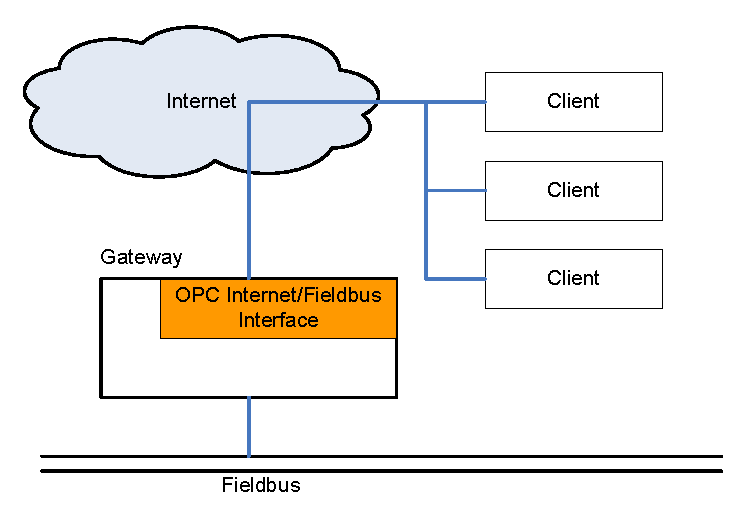
\includegraphics[scale=0.7]{graphics/inet_fb_gw.eps}
\caption{Internet/fieldbus interface on a gateway}
\label {inet_fb_gw} 
\end{figure} 

Historically, OPC used the Distributed Component Object Model (DCOM)
for the underlying communication technology. DCOM has the disadvantage
of being platform specific: it is only available for Microsoft
Windows based systems. Other platforms, such as Linux, can therefore
not retrieve fieldbus data from DCOM based servers. Another
disadvantage of DCOM is that it can not easily bypass firewalls, hence
access will often be limited to certain segments of a corporate
network.

In the last years, a new technology, called SOAP Web services, emerged.
\cite{SOAP2} defines a Web Service as: ``a method or function that is
available for other applications to access over the Internet.''. Web
services enable Remote Procedure Calls (RPC) and have the following
key features:

\begin{description}
\item[High level of interoperability:] Web services technologies are
all based on strictly defined open standards\footnote{Most
technologies are W3C standards.}.
\item[High networking abilities:] As an underlying communication
protocol, Web services utilize Internet protocols such as the Hyper
Text Transfer Protocol (HTTP) or the Simple Mail Transfer Protocol
(SMTP). These protocols have high networking abilities and may
moreover penetrate firewalls.
\item[Protocol legible by humans:] The Simple Object Access Protocol
(SOAP)\footnote{To be correct, SOAP is not an acronym for Simple
Object Access Protocol anymore, instead it's simply ``SOAP''.} is based
on the Extended Markup Language (XML), which is legible to
humans. This way, testing and debugging of Web services is far easier
than with binary protocols.
\item[Documentation:] Another underlying technology of SOAP is the
``Web Service Definition Language'' (WSDL) which may be used to define
the service, especially by constraining the format of the SOAP
protocol. WSDL utilizes the XML Schema language for defining these
SOAP messages\footnote{More information about XML Schema can be found
in \cite{XSD1}.}. These WSDL documents can be utilized by frameworks
to generate stubs that provide a base for accessing a Web service.
\item[Validation:] WSDL in combination with a validating XML parser
enable the validation of SOAP messages. This way, custom code will
never receive syntactically or semantically erroneous data, which
should improve the stability of the service.
\end{description}

SOAP Web services are seen as a successor to several alternative
technologies such as DCOM and are already broadly accepted by the
industry. More information about the SOAP protocol can be found in
\cite{SOAP1} and \cite{SOAP2}.

The OPC consortium reacted on this technological evolution by adopting
SOAP Web services for their standards. One recent addition of OPC is
the "XML Data Access Version 1.0" (XML-DA 1.0) standard. This standard
deals with access of underlying fieldbus technologies and covers the
following aspects:

\begin{description}
\item[Information model:] The specification provides a simple
information model, based on ``OPC Items'' which represent a piece of
information, similar to fieldbus data points. These items can be
arranged hierarchically.
\item[Data types:] OPC XML-DA adopts several XML-Schema based data
types, such as integer, float, date/time specific types. Moreover it
defines arrays which are based on these basic types.
\item[Operations:] The standard specifies 8 operations such as
reading/writing and browsing which can be used to access the
underlying fieldbus.
\item[Subscription:] The specification further introduces a mechanism
to retrieve only changed items, called ``Subscription''.  Clients may
thus subscribe to items and use a dedicated polling operation to
retrieve changed data.
\end{description}

The standard does not address security, instead it relies on
underlying Web service technologies\footnote{For instance, HTTPS can
be used to secure a HTTP channel.}. More information about OPC XML-DA
can be found in \cite{diplomarbeit} and \cite{OPCXMLDA}.

Although OPC XML-DA is based on open and standardized technologies, it
can nevertheless be tedious to build services based on this standard.
Therefore several OPC frameworks are available that introduce simple
building of client and server applications. However, most of these
frameworks are not freely available, moreover most of them are based
on Microsoft's .Net framework and are therefore platform dependent.

Due to these limitations, the PyOPC framework was developed, which
fully implements the OPC XML-DA standard, enabling developers to build
OPC XML-DA based applications in an easy way.

\newpage

%% 2 Introduction
%% Description: 
%%
%%

\section {Installation/Quickstart}
\thispagestyle{plain}

Before installing the PyOPC framework, the following three software
packages have to be installed:

\begin{description}
\item[Python:] The Python programming language can be downloaded from
http://www.python.org. It is available for a variety of operating systems.
{\bf The Python version must be at least 2.4.}

\item[Zolera Soap Infrastructure (ZSI):] The ZSI framework is used for
parsing and generating the SOAP messages. It is available from
http://pywebsvcs.sourceforge.net/. ZSI is still under development, therefore
different releases may not work. The ZSI-2.0\_rc3 release is known to work
with PyOPC.

\item[Twisted:] The Twisted server framework is used for the server
functionality. It is available from http://twistedmatrix.com/. All
recently released versions should be appropriate.
\end{description}

Installation instructions for the above software packages should be
available at the given websites.

PyOPC does currently not have an installer but is nevertheless
relatively easy to install. At first the PyOPC package has to be
decompressed. Then Python has to be informed where to find it. This is
done by adding the location of the PyOPC variable to the environment
variable {\sl PYTHONPATH}.

If everything is installed correctly, the next step may be to test the
installation. PyOPC contains extensive unit tests in the subdirectory ``test''.
These tests can either be run altogether by executing ``runtests.sh'' or 
selectively via the ``trial'' command from the Twisted framework. Hopefully,
all tests will pass\footnote{On some slower machines, certain server operations
may fail as they rely on a predefined execution time of certain operations.}. 

If all goes well, PyOPC is ready to use. As a quickstart, an existing
OPC XML-DA server may be queried directly from python such as shown in
listing \ref{ex_quickstart}\footnote{A demo server, implemented with
PyOPC, is set up at http://violin.qwer.tk:8000/, which may, however,
not be available all the time. There are several other public OPC
XML-DA compliant servers available. Some addresses for such servers
may be found at http://www.opcfoundation.org, moreover Advosol also
offers access to some demo servers (see http://www.advosol.com).}.

\lstset{language=C}
\begin{lstlisting}[caption={Accessing a remote OPC XML-DA server}
                   ,label=ex_quickstart] 
from PyOPC.XDAClient import XDAClient

address='http://path/to/server'
xda = XDAClient(OPCServerAddress=address)
xda.GetStatus()
\end{lstlisting}


\newpage

%% 3 Basic PyOPC concepts
%% Description: 
%%
%%

\section {Architecture and Basic Concepts}

The PyOPC framework supports the rapid development of OPC XML-DA compliant
clients and servers and provides the following features:

\begin{description}
\item[Open source:] PyOPC and all underlying technologies are
open source projects.

\item[Multi-platform capable:] The underlying programming language of
PyOPC is Python, which is available on most platforms, such as
Microsoft Windows, Linux, Mac OS X and others. Applications built with
PyOPC can be run on all platforms with Python support. A good
introduction to the Python programming language can be found in
\cite{diveintopython} and \cite{PYTHON}.

\item[Ease of use:] Various complex functionality of the OPC XML-DA
specification is automatically handled by the PyOPC framework,
therefore the developer does not need to cope with it. Nevertheless,
the programmer may also choose to override this functionality and
thus implement it in his own way.

\item[Extensible and reusable:] Basic framework functionality
can be extended by the programmer, moreover, OPC servers built with
PyOPC can be added to the framework as a custom libraries, which can
then be reused by other applications.
\end{description}

An OPC XML-DA compliant framework needs to support several
technologies, especially building servers which process concurrent
requests and handle the SOAP and HTTP protocol. Although Python has an
extensive collection of libraries, it does not fulfill these
requirements. Therefore two additional Python frameworks are used,
which have to be available on systems that provide PyOPC based
applications. These basic technologies are illustrated in figure
\ref{technologies}.

\begin{figure}[ht]
\htmlborder{1}
\centering
\includegraphics[scale=0.7]{graphics/technologies.eps}
\caption{Underlying Technologies of the PyOPC Framework}
\label {technologies} 
\end{figure}

\begin{description}
\item[Zolera Soap Infrastructure (ZSI):] This SOAP framework enables
parsing and serializing SOAP messages. PyOPC uses ZSI to read and
create OPC XML-DA compliant SOAP messages\footnote{This process is
hidden from developers, instead PyOPC provides abstract Python objects
for accessing underlying SOAP messages.}.

\item[Twisted:] Twisted is an asynchronous client/server framework.
It implements a variety of Internet protocols, such as HTTP and SMTP
and uses an event based mechanism to enable the development of
clients and servers which can handle concurrent requests.

In order to develop applications with Twisted, the programmer has
to lay out his program according to this event-based architecture.
Therefore building complex server applications with PyOPC require
some understanding of the basic concepts of Twisted. More information
about this framework can be found at \cite{TWISTED}.
\end{description}

\subsection {Basic PyOPC Architecture}

The PyOPC framework supports the development of OPC XML-DA client and
server applications. The OPC XML-DA standard defines the following
eight operations, which can be used to access OPC data:

\begin{description}
\item[GetStatus:] This operation is used to retrieve status information of
the OPC server.
\item[Read/Write:] These operations are used to read and write OPC
items\footnote{OPC items are basically containers which may hold a
piece of information. They resemble fieldbus data points and may
contain arbitrary data.}.
\item[Subscribe / SubscriptionPolledRequest / SubscriptionCancel:]
These operations are used to handle OPC subscriptions.
\item[Browse:] This operation is used to browse OPC items.
\item[GetProperties:] OPC items have so-called properties, which
define and describe the item. GetProperties can be used to retrieve
these OPC item properties.
\end{description}

Associated to each of these operation is a request and response SOAP
message, resulting in 16 different messages. With ZSI, these messages
can be parsed and serialized through specific Python objects,
so-called ``Typecodes''. Although accessing typecodes is far easier
than accessing the SOAP message itself, it is still a tedious
task. Therefore PyOPC hides this process from the developer by
defining various methods, which automatically handle the ZSI
typecodes. 

PyOPC introduces several classes, which are used throughout the
framework. These classes inherit from each other, forming a class
hierarchy, as illustrated in figure \ref{object_hierarchy}.

\begin{figure}[ht]
\htmlborder{1}
\centering
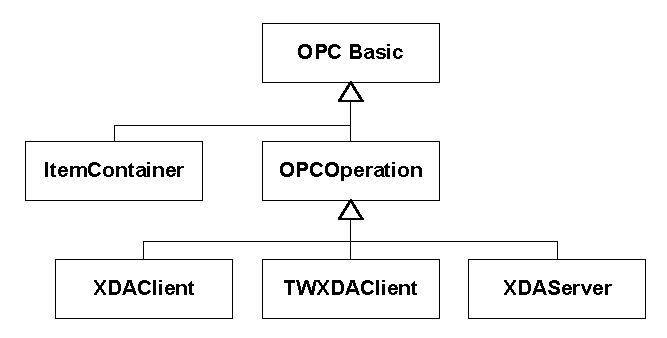
\includegraphics[scale=0.7]{graphics/object_hierarchy.eps}
\caption{Class Hierarchy of the PyOPC Framework}
\label {object_hierarchy} 
\end{figure}

The classes of this hierarchy implement the following functionality:

\begin{description}
\item[OPC Basic:] This class implements basic issues that are used by
other inheriting classes. Apart from several utility methods, the
class defines all OPC errors.
\item[OPCOperation:] The OPCOperation class handles the generation and
parsing of all OPC XML-DA SOAP messages. The class implements two read
and write methods for each operation\footnote{Every request and
response SOAP message has each a read and write method.}, which are
automatically utilized for handling ZSI typecodes.
\item[ItemContainer:] This class represents OPC items and is
described in detail below.
\item[XDAClient:] Simple OPC XML-DA clients may be built with this
class.
\item[TWXDAClient:] This class is an advanced way to build OPC XML-DA
compliant clients. The TWXDAClient class utilizes Twisted to enable
multiple, concurrent client requests.
\item[XDAServer:] The XDAServer class is the base to implement OPC
XML-DA compliant servers with the PyOPC framework.
\end{description}

\subsection {Representation of OPC XML-DA Data with Python Objects}

As already mentioned, handling SOAP messages with ZSI is not
simple. Therefore specific objects are defined by PyOPC which can be
easily accessed and represent the corresponding SOAP messages.

OPC XML-DA compliant SOAP messages contain various options which may
either concern the whole operation (global options) or may be item
specific (local options).  After closely examining these messages, it
was found that these options can be mapped to two certain Python
objects as depicted in figure \ref{message_basic}.

\begin{figure}[ht]
\htmlborder{1}
\centering
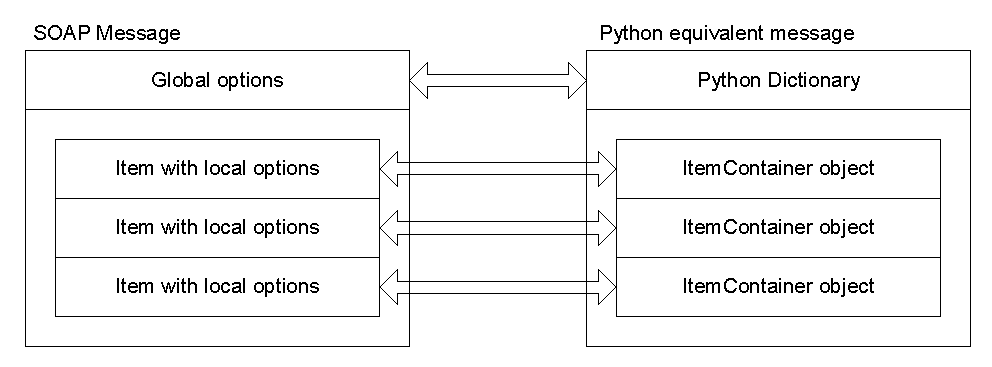
\includegraphics[scale=0.7]{graphics/message_basic.eps}
\caption{Python Objects Representing OPC XML-DA Messages}
\label {message_basic} 
\end{figure}

These two Python objects are the basic containers in the PyOPC
framework and are used to transport OPC data. Therefore they are used
as parameters for methods which represent OPC XML-DA operations.
Listing \ref{ex_message_basic} shows an example of an OPC XML-DA read
operation.

\lstset{language=C}
\begin{lstlisting}[caption={Usage of Python objects for representing
global and local options of a OPC XML-DA compliant SOAP message}
                   ,label=ex_message_basic] 
item = ItemContainer(ItemName='test_name', MaxAge=500)
item_list,global_options = xda.Read([item], ItemPath='test_path')
\end{lstlisting}

In line 1, an ItemContainer object is created, which contains the item
specific (local) options ``ItemName'' and ``MaxAge''. In line 2 the
read operation is taking place, with a list of ItemContainer objects
as the first parameter and the global option ``ItemPath'' as the
second.  The results of the read operation also consist of a list of
ItemContainer objects and a Python dictionary, containing the local
and global options.

Global and local options may sometimes be the same. In this case, the
local options override the global ones. For instance, if the option
``ItemPath'' is specified globally and locally, the local, item
specific ItemPath will have precedence.

As this mechanism is the same for all operations, it is sometimes
possible to set options that have no meaning for the current
operation. However, only relevant options will be included in the
resulting SOAP message, other options are ignored by the PyOPC
framework.  For instance, setting the option ``MaxAge'' for an OPC
Write operation has no effect at all.

There are a number of options that can be set for OPC XML-DA
operations, which can be looked up in \cite{OPCXMLDA}. These options
are case sensitive, for instance ``MaxAge'' and ``maxage'' are handled
as a different option.


\subsubsection*{Global OPC XML-DA options}

Python dictionaries are used to represent global options. As denoted
above, these dictionaries can then be used as parameters for OPC
operations.  However, often it is handy to define default global
options that are used all over the application. For instance, it may
make sense to define a server-specific default ``MaxAge'' option,
which is automatically assigned to all according SOAP messages.

Therefore PyOPC allows to specify these global options at the creation
of the client or server object, such as shown in listing \ref{ex_global}.
These global options will then be used for all operations, unless they
are overridden by global options in the method parameters.

\lstset{language=C}
\begin{lstlisting}[caption={Assigning Global Options to a PyOPC 
Client Instance}
                   ,label=ex_global]
xda = XDAClient(ReturnErrorText=False,
                ReturnItemName=True,
                ReturnDiagnosticInfo=True,
                ItemPath='')
\end{lstlisting}

The PyOPC framework always checks if global options, which are passed
as method parameters, can be applied to the current OPC operation. If
an option is unknown or misspelled, a Python {\sl TypeError} will be
raised. This way, errors due to accidental misspellings or improper
use of options are prevented.

\subsubsection*{The ItemContainer Object}

The ItemContainer object is used to store all local, item-specific OPC
XML-DA data, such as the item value and item-specific local
options. This information is stored in the object as object attributes
and may be accessed as shown in listing \ref{ex_itemcontainer}.


\lstset{language=C}
\begin{lstlisting}[caption={Accessing the PyOPC ItemContainer Object}
                   ,label=ex_itemcontainer] 
from PyOPC.OPCContainers import *
item = ItemContainer(ItemName='test_name',
                     MaxAge=500)
item.ItemName='other_name'
maxage = item.MaxAge
\end{lstlisting}

At the beginning of the example listing, the appropriate Python module
is imported that contains the ItemContainer class. In line 2, item
specific options are set at initialization time of the ItemContainer
object, while line 4 and 5 show how to directly set and retrieve
object attributes.

\cite{OPCXMLDA} defines numerous, sometimes complex local
options. Therefore errors due to misspellings can easily happen. To
prevent such errors, the ItemContainer class defines all possible
options via class attributes. In addition, an ItemContainer object
will not allow the setting of undefined object attributes. If the
developer accidentally tries to set a misspelled or unknown attribute,
the PyOPC framework raises a Python AttributeError.

\subsubsection*{Qualified Names (QNames) and Namespaces}

The OPC XML-DA specification and its associated SOAP messages
sometimes contain {\sl Qualified Names} (QNames). QNames consist of a
namespace, most often in the form of an Uniform Resource Locator (URL)
and a name. For this purpose, PyOPC defines a simple {\sl QName}
object, which is similar to a Python tuple.

Moreover PyOPC defines in the module {\sl utils} the following global
variables which may be used as the namespace part for QNames:

\begin{itemize}
\item{\sl NS\_XSD}, the namespace for XML-Schema
\item{\sl NS\_ZSI}, the ZSI namespace
\item{\sl NS\_XDA}, the namespace of the OPC XML-DA specification
\item{\sl NS\_PYO}, the PyOPC namespace
\end{itemize}

An example how to create and access such a QName object is given
in example \ref{ex_qnames}, showing the creation of a predefined 
and a custom QName in line 3 and 4 and accessing parts of the
QName in line 5:

\lstset{language=C}
\begin{lstlisting}[caption={Handling Qualified Names (QNames) with PyOPC}
                   ,label=ex_qnames] 
from PyOPC.utils import *

qn1 = QName(NS\_XSD,'string')
qn2 = QName('http://my/name/space','test123')
url, name = qn2.URI, qn2.name
\end{lstlisting}

\subsubsection*{OPC Item Properties}

Every OPC Item may have so-called {\sl properties} that contain
further information about the item. Example properties would be the
access rights or a description of the item. These OPC properties are
modeled as a specific Python object, called {\sl OPCProperty}, which
contains the following information:

\begin{description}
\item[Name:] The name uniquely identifies an OPC property. Names must
be of the type {\sl QName}.
\item[Value:] Properties most often have a value, for instance in case
of a property ``accessRights'', it stores the strings {\sl readable}
or {\sl writable}.
\item[Description:] In order to easily understand the meaning of a 
property, it can store a description.
\item[ItemPath/ItemName:] The address of the property, consisting of
the ItemPath and ItemName. 
\item[ResultID/ErrorText:] In case a property is erroneous, for
instance if it cannot be read or does not exist, the error can be
stored in a ResultID and a descriptive error text.
\end{description}

Listing \ref{ex_properties} shows in line 1 to 5 how to create and
access a PyOPC property object.

\lstset{language=C}
\begin{lstlisting}[caption={Creating and Accessing PyOPC Properties}
                   ,label=ex_properties] 
p1 = OPCProperty(Name = QName(NS_XDA,'accessRights'),
                 Value = 'readable',
                 Description = 'Access Rights')
print p1.Name, p1.Value
p1.ItemPath = 'MyPath'                 

p2 = OPCProperty(Name = 'accessRights')
print p2.Description
\end{lstlisting}

The OPC XML-DA standard specifies various common properties, which
should be preferred over custom properties, if possible. A full list
of these available properties is given in \cite{OPCXMLDA}. The alternative
are custom properties that will often be in the namespace of
PyOPC. Therefore the framework offers a simple shortcut in creating
properties: if the property name is a string instead of a QName, PyOPC
searches in a table for a matching OPC property.  If one is found, the
OPC XML-DA namespace is used, moreover the description is filled out
automatically. If the property is unknown, the PyOPC namespace will
automatically be used. This behavior is reflected in line 7 and 8 in
listing \ref{ex_properties}.

Properties will be associated with items, therefore an ItemContainer
object provides the following methods to add, delete and list
properties:

\begin{itemize}
\item{\sl addProperty(self, property) /
addProperties(self,properties)} adds one property or a list of
properties to the ItemContainer object.
\item{\sl getProperty(self, name)} retrieves a property according to
its name
\item{\sl delProperty(self, name) / popProperty (self, name)} deletes
a property. {\sl popProperty} returns the property before deletion.
\item{\sl listProperties(self)} returns a list of all item properties.
\end{itemize}


\subsubsection*{Representation of the Item Value with PyOPC Data Types}

OPC items have a {\sl value}, containing the actual information, which
corresponds to the value of a fieldbus data point. This value will be
of a certain OPC data type, such as string or integer but also more
complex types, such as an array. In order to access this information,
PyOPC has to map the OPC data type to a corresponding Python data
type, resulting in a possible data conversion. Table \ref{dataconv}
describes all possible data conversions.

\begin{table}[ht]
\htmlborder{1}
\centering
\includegraphics[scale=0.7]{graphics/dataconv.eps}
\caption{Data Conversion Between OPC XML-DA and PyOPC}
\label{dataconv} 
\end{table}

Currently, the following data types are not supported by the PyOPC
framework\footnote{The reason for these unsupported data types is that
the underlying SOAP framework, ZSI, does also not support them.}:

\begin{itemize}
\item The {\sl decimal} data type is currently not supported at all and
cannot be used.
\item The time based data types are not fully supported. Instead of
using Pythons datetime module, all data types are converted to the
Python time type. The duration type cannot be used. During conversion,
fractions of seconds and the time zone is lost.
\item The base64Binary type is mapped to a Python string. It may be
reasonable to use a corresponding Python type instead, however this is
currently not supported.
\end{itemize}

\cite{OPCXMLDA} further defines arrays, which may contain OPC data
types from the above. These arrays are directly mapped to Python
lists\footnote{OPC XML-DA further allows to nest arrays in arrays,
however this is currently not supported by PyOPC} and its elements are
converted as shown in Table 1.

\subsection{Error Handling}

OPC XML-DA describes the following two basic error types:

\begin{itemize}
\item OPC item specific, denoting that an OPC item is not
accessible or is unknown
\item OPC operation specific, identifying errors that concern the
whole operation
\end{itemize}

These two errors are handled entirely different in both OPC XML-DA and
PyOPC.

\subsubsection*{OPC Item Specific Errors}

If an OPC item cannot be read, written, is unknown or is in any other
way erroneous, the OPC server has to inform the client. These errors
do not regard the whole operation, instead the response message, which
transports the OPC items, implements the two following options that
denote the item specific error:

\begin{description}
\item[ResultID:] Item specific errors are always outlined by the
ResultID. The OPC XML-DA specification distinguishes between so-called
error and success codes, denoting if the transported item data is
valid or not. The ResultID is of the type {\sl QName} and contains a
unique ID of the error. \cite{OPCXMLDA} defines various errors, which
are in the format of {\sl E\_FAIL} or {\sl E\_ACCESS\_DENIED}.  A
complete description of these error and success codes can be found in
\cite{OPCXMLDA}.

In case the provided OPC errors do not suffice, custom errors can be
defined. PyOPC defines a few errors in its namespace, which can also
be utilized.

\item[ErrorText:] This non-mandatory option may provide descriptive
error text, which will make the reason of an error understandable to
humans.

\end{description}

Despite of an item specific error, the response message may transport
invalid item data. Therefore OPC XML-DA applications always have to
check for the ResultID, so that item specific errors are detected.

\subsubsection*{OPC Operation Specific Errors}

If the whole operation fails, for instance if the server is busy or
malfunctioning, or if the client request is badly formatted, the
server responds with a SOAP Fault message, which contains a detailed
error description.

SOAP Faults are caught by the ZSI framework. This way PyOPC can raise
an OPC specific Python error, the {\sl OPCServerError}. The
OPCServerError inherits from ZSI's {\sl Fault} error and contains the
SOAP faultcode, the faultstring and the detail. More information about
SOAP faults can be found in \cite{SOAP1} or \cite{SOAP2}.

\thispagestyle{plain}

\newpage

%% 4 Client specifics
%% Description: 
%%
%%

\section {Client Functionality}
\thispagestyle{plain}

The PyOPC framework enables access of OPC XML-DA compliant servers by
providing classes that can be used to easily create OPC XML-DA
clients.

PyOPC offers two different classes for this task:

\begin{itemize}
\item The {\sl XDAClient} class that implements simple access of OPC
servers. This class does not offer concurrent connections.

\item PyOPC also provides the more complicated {\sl TWXDAClient}
class, which is based on the Twisted framework. {\sl TWXDAClient}
enables concurrent client connections by utilizing Twisted's event
mechanism.
\end{itemize}

These classes are contained in two different Python modules, namely
{\sl XDAClient} and {\sl TWXDAClient}) that have to be imported before
the client classes can be used. As already shown in Listing
\ref{ex_global}, global options can be defined during object creation,
which then apply to all OPC operations that are handled by this client
object.

Most of these options are OPC-specific and are described in
\cite{OPCXMLDA}.  However, the following options are PyOPC-specific or are 
automatically handled by the client object:

\begin{description}
\item[OPCServerAddress:] This option specifies the address of the OPC
XML-DA server, such as {\sl http://path/to/server}. The
OPCServerAddress option is mandatory and can only be applied during
client object creation.

\item[ClientRequestHandle/ClientItemHandle:] These options may help
the OPC client and server to distinguish between different client
requests. If these options are not specified, they will be
automatically generated by PyOPC.
\end{description}

%% All PyOPC-based twisted clients log the SOAP messages to a file called
%% ``soap.log'' in the current working directory. This file can be
%% utilized by developers to debug certain problems.

\subsection{Building OPC XML-DA Clients with the PyOPC XDAClient class}

Listing \ref{ex_xdaclient} shows example code of a PyOPC
XDAClient-based client\footnote{This sample code can also be found in
the file {\sl samples/clients/simple.py} in the PyOPC distribution}
that first retrieves the server status, browses the root item and
reads an item:


\lstset{language=C}
\begin{lstlisting}[caption={Sample client code based on the PyOPC XDAClient 
module}
                   ,label=ex_xdaclient] 
from PyOPC.OPCContainers import *
from PyOPC.XDAClient import XDAClient

def print_options((ilist,options)):
    print ilist; print options; print
    
address='http://violin.qwer.tk:8000/'

xda = XDAClient(OPCServerAddress=address,
                ReturnErrorText=True)

print_options(xda.GetStatus())
print_options(xda.Browse())
print_options(xda.Read([ItemContainer(ItemName='simple_item', 
                                      MaxAge=500)], 
                       LocaleID='en-us'))
\end{lstlisting}

Line 1 and 2 import the needed PyOPC modules. In Line 4 a simple function
is defined that prints a list of ItemContainer objects ({\sl ilist}) and
the global options Python dictionary ({\sl Options}).

In line 9, the client object is created: As global options, the server
address is specified and {\sl ReturnErrorText = True} denotes that the
client requests verbose error descriptions.

Lines 12, 13 and 14 show the three different OPC operations. The
return parameters of these operations are a list of ItemContainer
objects and the global options (a Python dictionary), which are both
handled by the function {\sl print\_options}.

\subsection{Building OPC XML-DA Clients with the PyOPC TWXDAClient class}

The {\sl XDAClient} module has the disadvantage that operations can
only be handled sequentially. When certain OPC operations take
significantly longer than others, it is a better solution to execute
the requests in parallel. The Twisted framework introduces an
event-based mechanism that is utilized by the the {\sl TWXDAClient},
so that concurrent server requests can be made\footnote{This
event-based mechanism must not be confused with
multi-threading.}. However, this Twisted-based client class is more
complex than its simpler alternative. More information about the
Twisted framework and its underlying concepts can be found in
\cite{TWISTED}.

Listing \ref{ex_twxdaclient} implements the same functionality as 
listing \ref{ex_xdaclient} but executes the three OPC operations 
concurrently:

\lstset{language=C}
\begin{lstlisting}[caption={Sample client code based on the PyOPC TWXDAClient 
module}
                   ,label=ex_twxdaclient] 
from PyOPC.OPCContainers import *
from PyOPC.TWXDAClient import TWXDAClient
from twisted.internet import reactor

OPERATIONS = 3

def print_options((ilist,options)):
    print ilist; print options; print
    global OPERATIONS
    OPERATIONS -= 1
    if OPERATIONS == 0:
        reactor.stop()

def handleError(failure):
    print "An Error occured"
    print failure.getTraceback()
    reactor.stop()
    
address='http://violin.qwer.tk:8000/'

xda = TWXDAClient(OPCServerAddress=address,
                ReturnErrorText=True)

d = xda.twGetStatus()
d.addCallback(print_options)
d.addErrback(handleError)

d = xda.twBrowse()
d.addCallback(print_options)
d.addErrback(handleError)

d = xda.twRead([ItemContainer(ItemName='simple_item', MaxAge=500)],
               LocaleID='en-us')
d.addCallback(print_options)
d.addErrback(handleError)

reactor.run()
\end{lstlisting}

In line 3, certain Twisted modules are imported. Line 24-26 show how
an OPC operation is done in ``Twisted style'': first, the method {\sl
twGetStatus} is called that returns a deferred. Then two functions are
attached to this deferred, namely a ``callback'' method, which prints
the results of the OPC operation and an ``errback'' method, which is
executed when an error (failure) is returned.

In line 37, all deferreds are initialized, therefore the Twisted
reactor is started, which triggers all deferreds. This way, all OPC
operations are started and when the requested data is returned, the
appropriate callback/errback methods are called.

As the execution order of the attached callback methods cannot be
predicted, a global variable {\sl OPERATIONS} is defined, which is
used by the function {\sl print\_options} to stop the Twisted reactor
when all pending server requests have finished.


\newpage

%% 5 Server specifics
%% Description: 
%%
%%

\section {Server Functionality}
\thispagestyle{plain}

The PyOPC framework also enables easy and rapid creation of OPC XML-DA
compliant servers. Implementing OPC servers is more complicated than
creating clients, however PyOPC introduces several concepts that
should greatly reduce the effort.

Most often, an OPC server will retrieve data from underlying devices
or networks, such as fieldbuses. Most of these underlying technologies
will also provide operations similar to OPC operations, such as
reading and writing. In such a situation, the OPC XML-DA server will
be similar to a proxy, which retrieves data on one side from
fieldbuses or devices, reformats it and provides it to clients on the
other side, such as depicted in figure \ref{opc_proxy}.

\begin{figure}[ht]
\htmlborder{1}
\centering
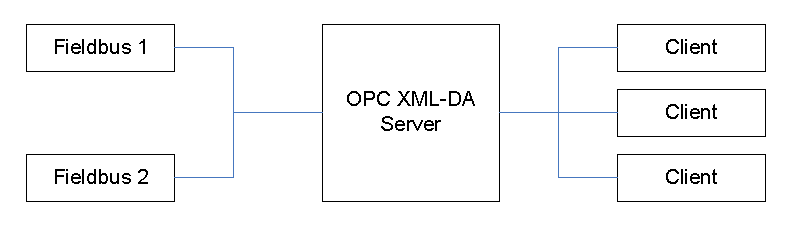
\includegraphics[scale=0.7]{graphics/opc_proxy.eps}
\caption{OPC XML-DA Server as a Proxy}
\label {opc_proxy} 
\end{figure}

PyOPC introduces a server class, the {\sl XDAServer}, which provides
methods for each OPC operation. This class can be inherited and the
methods can be overridden by custom implementations, as illustrated
in figure \ref{server_hierarchy}.

\begin{figure}[ht]
\htmlborder{1}
\centering
\includegraphics[scale=0.7]{graphics/server_hierarchy.eps}
\caption{Server Class Hierarchy}
\label {server_hierarchy} 
\end{figure}

For instance, the class {\sl BasicXDAServer} inherits from {\sl
XDAServer}.  The BasicXDAServer class overrides certain functionality
of its parent class, such as Read and Write, where it implements its
own functionality. However, this is still a quite general class and
is not intended for the actual server instance. Instead, another class,
{\sl MyBasicXDAServer} inherits from the class, which defines various
attributes that define the runtime parameters for the server instance,
such as ``GetStatus'', which may be set to any custom value.

This way, implementing a OPC XML-DA server with PyOPC leads to a three-level
class hierarchy:

\begin{enumerate}
\item The basic XDAServer class that implements general functionality, which
is provided by the PyOPC framework
\item A server-specific class that overrides certain operations to
implement its custom functionality, which has to be implemented for
the dedicated system
\item The production-specific class, which defines several production 
specific parameters and is used for the server instance.
\end{enumerate}

Listing \ref{ex_simple_server} shows the code for a very basic server
that inherits from the BasicXDAServer class, which enables to define
several OPC items in the server instance itself. These OPC items can
then be read and written by OPC clients.

\lstset{language=C}
\begin{lstlisting}[caption={Simple OPC XML-DA Server}
                   ,label=ex_simple_server] 
import random
from twisted.internet import reactor,defer
from PyOPC.servers.basic import BasicXDAServer

# Read sample OPC items for testing
import sample_items

class MyXDAServer(BasicXDAServer):
    OPCItems = sample_items.TestOPCItems
    StatusInfo = 'My Basic OPC XML-DA Server'

    def GetStatus(self, (IPH,inOptions,outOptions)):
        ''' Custom GetStatus that alters the Product Version'''

        outOptions['ProductVersion'] = str(random.choice(range(1,10)))
        
        return super(MyXDAServer, self).GetStatus((IPH,inOptions,outOptions))
\end{lstlisting}

In line 9 some predefined OPC items are set in the server instance. These
items are defined in an external module, which is imported in line 6.
Moreover the MyXDAServer class defines the class attribute ``StatusInfo''
which will then be used in the OPC ``GetStatus'' operation.

Line 12-18 shows how the ``GetStatus'' operation is overridden by the
inherited class. In this method, the OPC option ``Product Version'' is
set to an arbitrary number between 1 and 9.

Line 17 is very important: this line calls the method of the parent
class and returns the results. Python does not automatically call its
parent class, this has to be done manually.  However, it is mandatory
in PyOPC that an overridden OPC operation has to call the method in
its parent class. The reason is that this parent method fulfills
several needed functionality, such as setting several other needed OPC
options to maintain compatibility with the OPC XML-DA specification.
The call of the superclass method has always to be done at the
end of the custom method.

The above listing also shows how data such as the global options and
the OPC items are passed. It is obvious that any XDAServer-based
method, which represents an OPC operation, has to process parameters
from the client request message and has to create several appropriate
output parameters, which form the base of the response message. In
PyOPC, these request and response parameters are passed from one
method to another and thus also from each child to its parent method,
such as shown in figure \ref{opc_parameters}.

\begin{figure}[ht]
\htmlborder{1}
\centering
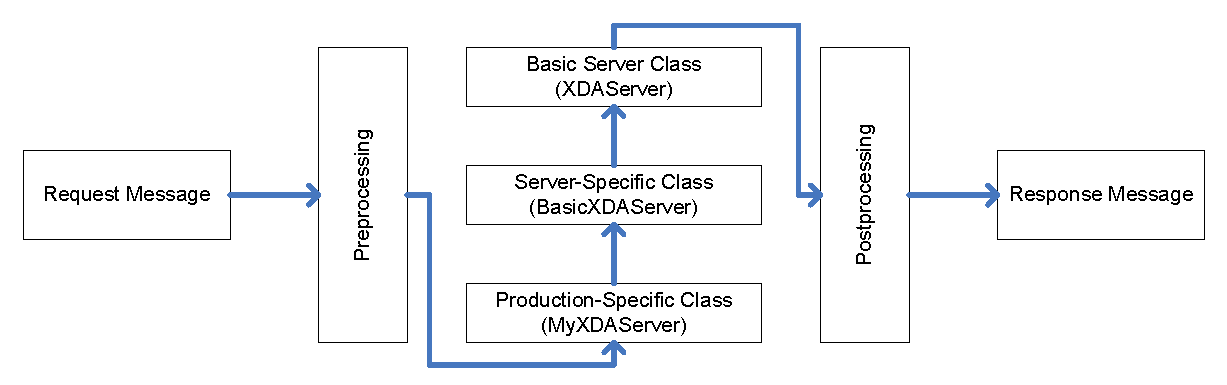
\includegraphics[scale=0.7]{graphics/opc_parameters.eps}
\caption{OPC Parameter Passing}
\label {opc_parameters} 
\end{figure}

Similar to the PyOPC-based client, the request and response messages
are represented by a Python dictionary that contains the global OPC
options and a list of ItemContainer objects, representing the OPC
items. It can be observed in figure \ref{opc_parameters} that 
OPC data is passed from one method to another. All these methods
require the input parameters and will set or alter certain output
parameters.

Therefore it is appropriate to aggregate the input and output
parameters in one Python object, which is then passed from one method
to another. Therefore each PyOPC method, which represents an OPC
operation, must define a Python tuple as a parameter which contains
the following three objects:

\begin{enumerate}
\item The {\bf Item Pair Holder} (IPH), a special object that contains
an input and output list of ItemContainer objects. These lists have
always to be of the same length and every input ItemContainer object
has a corresponding output ItemContainer object. These internal
ItemContainer lists are normally not directly accessed. Instead, the
ItemPairHolder object implements an ``append'' method, which can be
used to append an input and output ItemContainer object. Moreover the
object is iterable, which is most often needed by OPC operation
methods.

Listing \ref{ex_IPH} shows how such an ItemPairHolder can be created
and managed:

\lstset{language=C}
\begin{lstlisting}[caption={Creating and Managing the ItemPairHolder object}
                   ,label=ex_IPH] 
IPH = ItemPairHolder()
IPH.append(inItem, outItem)
for inItem, outItem in IPH:
   outItem.ItemPath = inItem.ItemPath
\end{lstlisting}

The example listing first creates an ItemPairHolder object and appends
some predefined ItemContainer objects. Then one certain attribute of
the output item, the ``ItemPath'' is set to its corresponding input
attribute.

\item The {\bf input options} (inOptions), a Python dictionary, which
contains all global input options
\item The {\bf output options} (outOptions), a Python dictionary, which
contains all global output options
\end{enumerate}

\subsection*{Server Configuration}

The server can be configured through several class attributes. These
attributes can either be overridden in the inheriting object, or can
also be specified at the server object instantiation.

The basic {\sl XDAServer} class provides the following options. (Their
default values are given in parentheses.) Some of them are are further
described in later sections:

\begin{description}

\item[AutoItemCache {\sl (True)}:] This option enables the automatic
OPC item caching.
\item[WritePurgeCache {\sl (True)}:] Denotes if the item cache should be
flushed after an item is written. 
\item[DefaultMaxAge {\sl (1000)}:] The default maximum age of an item.
\item[BufferSize {\sl (100)}:] The default subscription buffer size in
number of items.
\item[ThreadedParsing {\sl (True)}:] One of the most CPU-intensive
tasks is the parsing of the incoming SOAP message. In order to speed
up the server, it is possible to execute the parser in a separate
thread, so that the server can execute other requests in
parallel\footnote{The speed gain is currently not very significant, as
fast XML parsers are quite efficient compared to other tasks, such as
serializing the SOAP message.}.
\item[ThreadPoolSize {\sl (5)}:] The maximum amount of concurrent
threads.
\item[SubscriptionPingRate {\sl (10000)}:] The default subscription ping
rate in milliseconds.
\item[MaxPingRate {\sl (86400000 = 1 Day)}:] The maximum ping rate that
may be specified by a client.
\item[MaxSamplingRage {\sl (100)}:] The maximum sampling rate in
milliseconds that clients may specify.
\item[HandleProperty\_value/quality/timestamp/scanRate {\sl (True)}:]
Denotes if the above properties are automatically generated/handled.
\end{description}

\subsection{Preprocessing and Postprocessing}

The PyOPC XDAServer class automatically parses incoming SOAP messages
and creates appropriate PyOPC objects, which represent the incoming
message. After that, the preprocessing stage prepares and handles some
of the following options of the outgoing message:

\begin{description}

\item[RcvTime:] This option is set to the time, the SOAP message was
received by the server.
\item[ClientRequestHandle:] The content of the incoming
ClientRequestHandle is automatically copied to the outgoing message.
\item[RevisedLocaleID:] If the requested locale is not available, the
server automatically chooses the first available locale and returns it
with this options.
\item[ServerState:] This option is set to the ServerState attribute of
the server class, the default is ``running''.

\end{description}

After this stage, the server operation methods are executed.
Therefore the data from the preprocessing stage is available in these
methods and may be modified.  For instance, the read operation may
check for the option ``RevisedLocaleID'' in the outgoing message and
set it to a different locale.

After the server operations are finished, the PyOPC objects, which
represent the incoming and outgoing SOAP messages is handed over to
the postprocessing stage, which handles and modifies the following
options:

\begin{description}

\item[Unhandled Items:] As denoted above, the incoming and outgoing
OPC items are stored in the ItemPairHolder object. The preprocessing
stage will create this object, which contains an incoming
ItemContainer object and an associated, empty outgoing ItemContainer
object. The operations should then fill this outgoing item with
appropriate data. If, however, the outgoing ItemContainer object is
still empty\footnote{A ContainerItem is empty, if the attribute
'IsEmpty' is set to true. This happens if it is created such as
i=ItemContainer() and no attribute is ever set.} in the postprocessing
stage, an error of the type ``PYO\_E\_EMPTYITEM'' is associated with
it, denoting that the item contains no data.

\item[ErrorText:] If {\sl ReturnErrorText} is set to false in the
request message, any error text in the outgoing message is
deleted. Otherwise the error text will be kept, and if there is none
in the outgoing message, it will be set to a blank string.
\item[DiagnosticInfo:] If {\sl ReturnDiagnosticInfo} is set to false
or is omitted in the request message, any diagnostic info in the
outgoing message is deleted. Otherwise the diagnostic info will be
kept, and if there is none in the outgoing message, it will be set to
a blank string.
\item[Timestamp:] If {\sl ReturnItemTime} is set to false or is
omitted in the request message, any item-related timestamp in the
outgoing message is deleted. Otherwise the timestamp will be kept,
and if there is none in the outgoing message, it will be set to 
the current time.
\item[ItemPath/ItemName:] If {\sl ReturnItemPath/Name} is set to false
or is omitted in the request message, any ItemPath/Name in the
outgoing message is deleted. Otherwise the ItemPath/Name will be kept,
and if there is none in the outgoing message, it will be set to a
blank string.
\item[ClientItemHandle:] The ClientItemHandle of each incoming item is
copied to the according outgoing item.
\item[ReplyTime:] The ReplyTime in the outgoing message is set to the
current time, unless it has not been already set a previous server
method.

\end{description}

\subsection{Item Caching and Subscriptions}

PyOPC provides support for advanced OPC XML-DA services, such as 
subscriptions and Item Caching. Unless these services are disabled,
they are automatically available at any PyOPC-based OPC server.

\subsubsection*{Item Caching}

OPC XML-DA servers normally retrieve data from underlying systems,
such as fieldbuses. Different client will then access these items
through the OPC server. There may be situations, where many clients
access the same OPC item over and over. These client requests will
therefore lead to a significant load on underlying systems and may
even exceed their capabilities.

One solution to this problem is caching: when the OPC server retrieves
an item from an underlying system, it stores it for a predefined amount
of time. These cached items are then available for OPC clients, therefore
client requests do not necessarily lead to data retrieval from underlying
systems.

In the client request message, the option ``MaxAge'' may be specified,
denoting how old the item may be. If MaxAge is greater than the time
the item is cached, the server will build the response message upon
the cached item, otherwise the server will retrieve new data.

The PyOPC framework does automatically implement OPC item caching, if
the server attribute ``AutoItemCache'' is set to true (which it is by
default). The developer can also specify the attribute
``DefaultMaxAge'', which defines the maximum age in milliseconds for
requests that do not provide the MaxAge option.

The exact item caching mechanism is illustrated in figure
\ref{item_caching}:

\begin{figure}[ht]
\htmlborder{1}
\centering
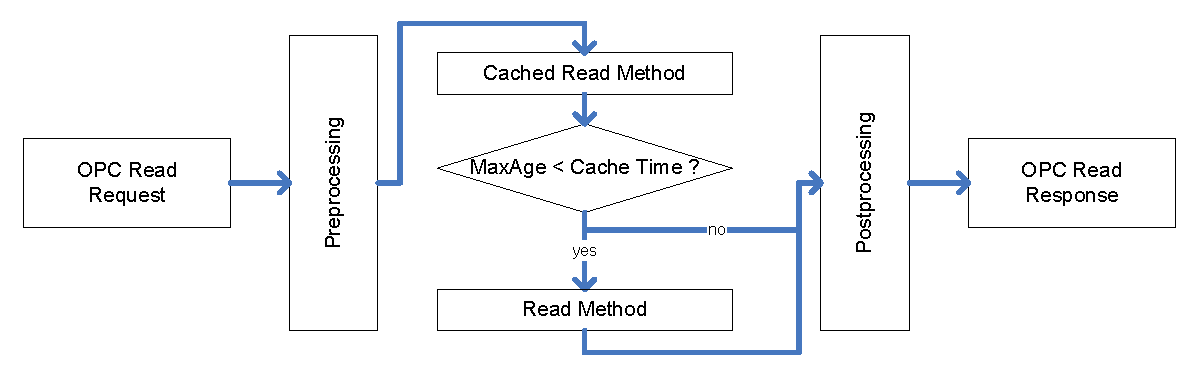
\includegraphics[scale=0.7]{graphics/item_caching.eps}
\caption{Mechanism of PyOPC Item Caching}
\label {item_caching} 
\end{figure}

If an OPC Read request message is received by the server and ``AutoItemCache''
is set to true, the XDAServer method ``CachedRead'' is called. This method
decides whether to return cached data regarding the MaxAge parameter or
whether it calls the server's read method, which retrieves the data from
the underlying system.

This way, the developer does not need to regard item caching, he has
to code only the data retrieval itself. His read method will be only called
if the maximum allowed age is smaller than the time, the item is cached.

Write operations update data in underlying devices. Therefore by
default the read cache of a written item is flushed. However, in
certain situations it may be appropriate not to clear the
cache. Therefore PyOPC provides the option ``WritePurgeCache'' which
can be set to false to omit the automatic cache flushing.

\subsubsection*{Subscriptions}

In order to observe OPC items, one could theoretically periodically
poll OPC items with read operations and check for changes. However,
such polling leads to an unnecessary network and server
load. Therefore \cite{OPCXMLDA} introduces so-called ``subscriptions''
and specifies three related OPC operations.

OPC clients may subscribe to items, which basically commands the
server to observe these items for changes. Such changes will be stored
by the server and can later be retrieved by the client.

Implementing such a subscription mechanism in the server is quite
complicated. The OPC XML-DA specification describes several complex
issues, such as deadband (recording items only if they exceeded a
predefined value) and the so-called extended subscription
architecture. A detailed description of these topics is given in
\cite{OPCXMLDA}.

To ease the development of OPC XML-DA servers, the PyOPC framework
implements a default mechanism for subscriptions which is
automatically available and functional for all OPC XML-DA servers
based on the {\sl XDAServer} class. The basic idea is that most
underlying systems such as fieldbuses have a read operation that is
roughly similar between different systems, while system notifications
- a common way to observe datapoints for changes - can be very
different on fieldbus systems. Therefore the most compatible way is to
utilize the read operation for subscriptions.

Therefore developers only have to implement the read operation and will
thus automatically enable subscriptions. The basic mechanism is illustrated
in figure \ref{pyopc_subs}.

\begin{figure}[ht]
\htmlborder{1}
\centering
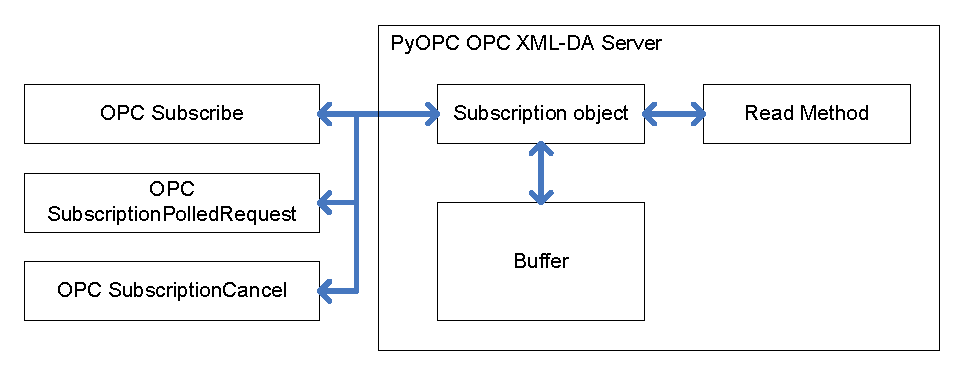
\includegraphics[scale=0.7]{graphics/pyopc_subs.eps}
\caption{Subscriptions in PyOPC}
\label {pyopc_subs} 
\end{figure}

It can be seen that a client can utilize the following three
operations to handle subscriptions:

\begin{itemize}
\item {\sl Subscribe} creates a subscription object in the server.
This subscription object will then utilize the server's read operation
to periodically poll the underlying system for changed items. These
changed items are then stored - either in the subscription object
itself, or, if specified by the client, in a subscription buffer,
which is shared among all subscriptions.
\item {\sl SubscriptionPolledRequest (SPR)} is then used by clients
to retrieve all changed values.
\item {\sl SubscriptionCancel} can then be used to cancel the subscription
which results in the deletion of the subscription object.
\end{itemize}

PyOPC also covers all complex subscription-related issues, such as the
PingRate, HoldTime/WaitTime, deadband and more, therefore developers
do not have to deal with these issues.

The following functionality can be configured in the server object:

\begin{description}
\item[BufferSize:] All OPC subscriptions share one buffer, which is
used to store changed items until they are fetched by the client via
the SPR operation. With the BufferSize attribute, the number of items
can be specified that the buffer can hold. If more items than this
number are stored in the buffer, the oldest entries are lost.
\item[SubscriptionPingRate:] If the client did not specify a ping
rate, this predefined value will be used. The ping rate defines, how
much time may elapse between two client polls. If the ping rate is
exceeded, the subscription is automatically canceled.
\item[MaxPingRate:] This is the maximum ping rate, a client may specify.
\item[MaxSamplingRate:] As denoted above, the subscription object
periodically fetches (samples) item values from underlying devices.
This sampling can be very demanding for the underlying system,
therefore a maximum sampling rate can be specified in the server. If a
client requests a higher sampling rate than this value, it is revised
to this value by the server.

OPC server developers should set this to a suitable value: the maximum
sampling rate should never be higher than the time that is needed for
a read request.
\end{description}

It should be denoted that PyOPC allows only one SPR for one
subscription object at a time. If a second concurrent SPR is issued,
the server will return an error\footnote{The OPC XML-DA specification
is quite loose on this topic, therefore in PyOPC concurrent SPRs are
prohibited.}.

An OPC server developer may also implement his own subscription
mechanisms. This can be done by overriding the three XDAServer methods
{\sl Subscribe, SubscriptionPolledRequest} and {\sl
SubscriptionCancel}, however, this will most often not be necessary.

\subsection{Operation Specific Functionality and Other Issues}

\subsubsection*{Automatic Readback}

In OPC write requests, the client may specify the option
``ReturnValuesOnReply''. If this option is set to true, the server
will read back the written values. This is accomplished by
calling the servers read method.

\subsubsection*{Browsing}

Clients may specify OPC properties in a browse request, which will
then be returned along with the appropriate browse result. In order to
retrieve these properties, the server's Browse method will call the
servers GetProperties method.

\subsubsection*{Property Handling}

Certain OPC properties, namely {\sl value, quality, timestamp} and
{\sl scanRate} can be automatically handled by the PyOPC
framework. This way, these four properties will be automatically
available for all OPC items.

The values of these properties will be retrieved as follows:

\begin{itemize}
\item The values of the {\sl value, quality} and {\sl timestamp} 
properties are simply retrieved with the servers read method,
which contains all needed data.
\item The value of {\sl scanRate} is set to MaxSamplingRate.
\end{itemize}

\subsubsection*{Logging}

PyOPC based servers also support detailed logging and provides the
following three different logs:

\begin{description}
\item[Access Logging:] If a client accesses the PyOPC server, the
clients IP address and the requested SOAPAction, which defines
the OPC operation is logged in this file. The default file name
for the access log is ``access.log''.
\item[Error Logging:] PyOPC server errors are kept in this log.
Its default name is ``error.log''.
\item[Debug Information:] During development and tests, it is often
interesting for the programmer to have access to further information,
especially to the client/server communication. Therefore PyOPC logs
the SOAP messages along with the HTTP header in a pretty-printed
style. By default the debug log is disabled.
\end{description}

The file names of these logs can be configure by setting the server
attributes ``access\_log\_fn'', ``error\_log\_fn'' and
``http\_log\_fn'' to the desired name. Moreover, logging can also be
omitted by setting one or more of these attributes to a blank string.

\subsubsection*{Setting Up an OPC Server Instance}

As the server classes of PyOPC are based on the Twisted framework, it
is also utilized to set up the OPC server instance. This can be done
as shown in listing \ref{ex_start}, which implies the proper
definition of the class ``MyXDAServer'', as already shown in listing
\ref{ex_simple_server}.

\lstset{language=C}
\begin{lstlisting}[caption={Instantiating and Starting a PyOPC-based
OPC XML-DA Server}
                   ,label=ex_start] 
from twisted.web import resource, server
xdasrv = MyXDAServer(http_log_fn = 'http.log')
root = resource.Resource()
root.putChild('',xdasrv)
site = server.Site(root)
reactor.listenTCP(8000, site)
reactor.run()
\end{lstlisting}

Line 1-2 import all needed Twisted modules and create the PyOPC
server object. In line 3, a Twisted resource object is created, where
servers can be added, such as shown in line 4. Line 5-7 then starts
the server. This server will then be reachable under the address
``http://server:8000/''.

A Twisted resource.Resource object is not limited to one PyOPC server
instance, instead it is possible to add multiple server objects, such
as shown in listing \ref{ex_multiserver}, which are then reachable
under different URLs.

\lstset{language=C}
\begin{lstlisting}[caption={Adding Multiple PyOPC Server Objects to
One Twisted Resource}
                   ,label=ex_multiserver] 
root = resource.Resource()
root.putChild('srv1',MyXDAServer1())
root.putChild('srv2',MyXDAServer2())
root.putChild('srv3',MyXDAServer3())
\end{lstlisting}

\subsection{Contributed Servers}

The PyOPC framework implements two simple servers, which on the one
hand can be seen as a reference design and may on the other hand be
used for setting up simple test servers.

\subsubsection*{BasicXDAServer}

This simple server does not retrieve data from other resources,
instead the OPC item data can be directly defined in the server.

Listing \ref{ex_basicxdaserver} shows the code of a server that is
based on the BasicXDAServer class:

\lstset{language=C}
\begin{lstlisting}[caption={PyOPC server based on the class 
BasicXDAServer}
                   ,label=ex_basicxdaserver] 
class MyXDAServer(BasicXDAServer):
    OPCItems = (ItemContainer(ItemName='sample_integer',
                               Value=14,
                               QualityField='good'),
                ItemContainer(ItemName='sample_float',
                               Value=96.43,
                               QualityField='good'))
\end{lstlisting}

This server defines two OPC items, which can then be accessed
by OPC XML-DA clients.

\subsubsection*{ESDProxy}

This server can be seen as a reference design for OPC servers that
retrieve OPC data from external sources. A detailed description of
this server can be found in \cite{diplomarbeit}.
\newpage

\begin{appendix}

s%% Description: Local/Global Options of OPC XML-DA
%%
%%


\section {Appendix A - Local/Global OPC Options}
\thispagestyle{plain}

The OPC XML-DA specification defines various options, which can be
global and/or local and are associated with one or more OPC operations.
A detailed description of these options can be found in \cite{OPCXMLDA}.
However, the specification is somehow complicated and some of these
options can not be easily found. Moreover these options will be 
represented by specific Python data types.

In order to ease the client/server development with PyOPC, table
\ref{operations1} and \ref{operations2} outline what options are
used by which functions. The letters ``G'' and ``L'' indicate if the
option is global or local for an OPC operation.

\begin{table}[!ht]
\htmlborder{1}
\centering
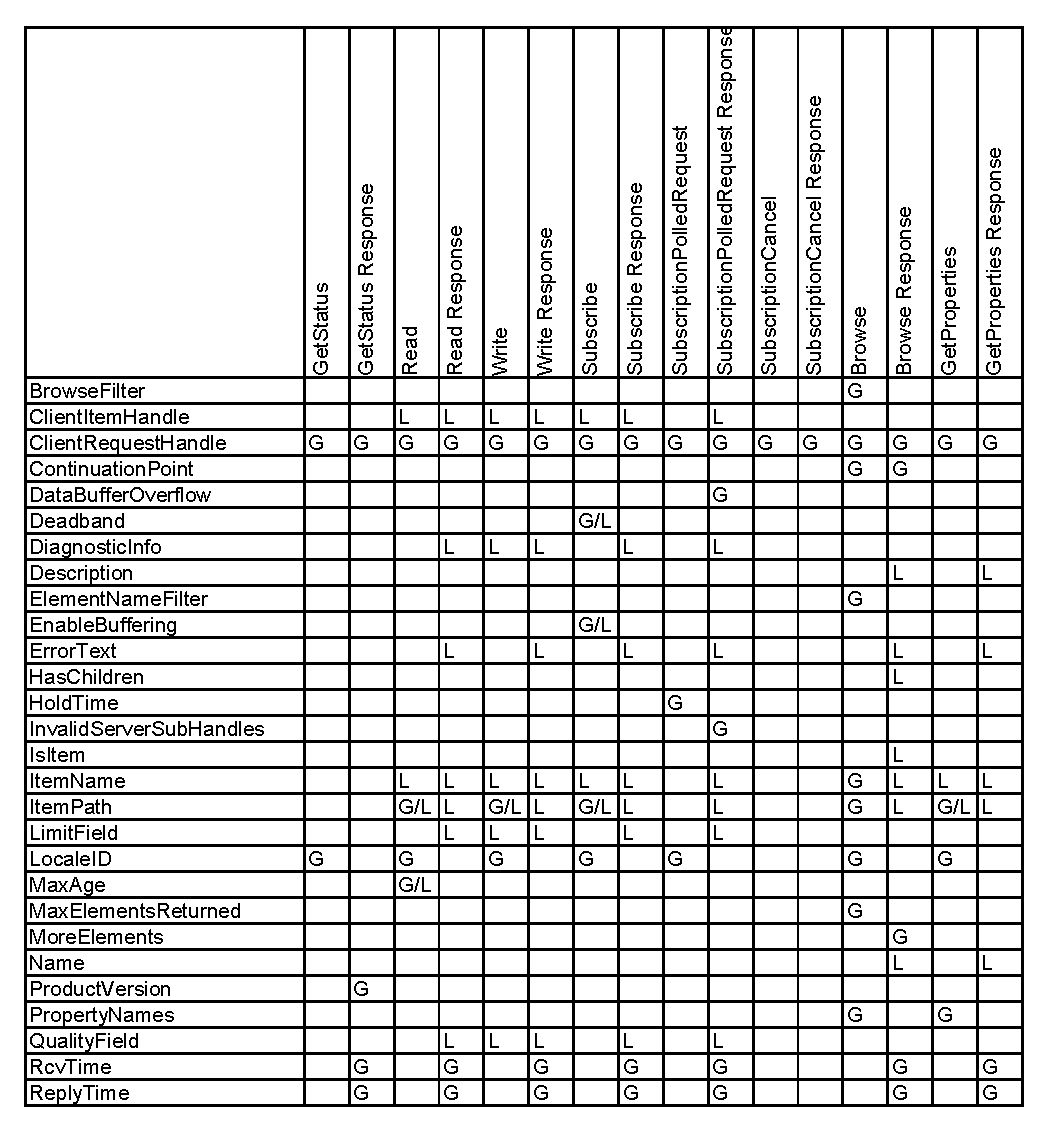
\includegraphics[scale=0.9]{graphics/operations1.eps}
\caption{OPC Options and Operations}
\label {operations1} 
\end{table}

\begin{table}[!ht]
\htmlborder{1}
\centering
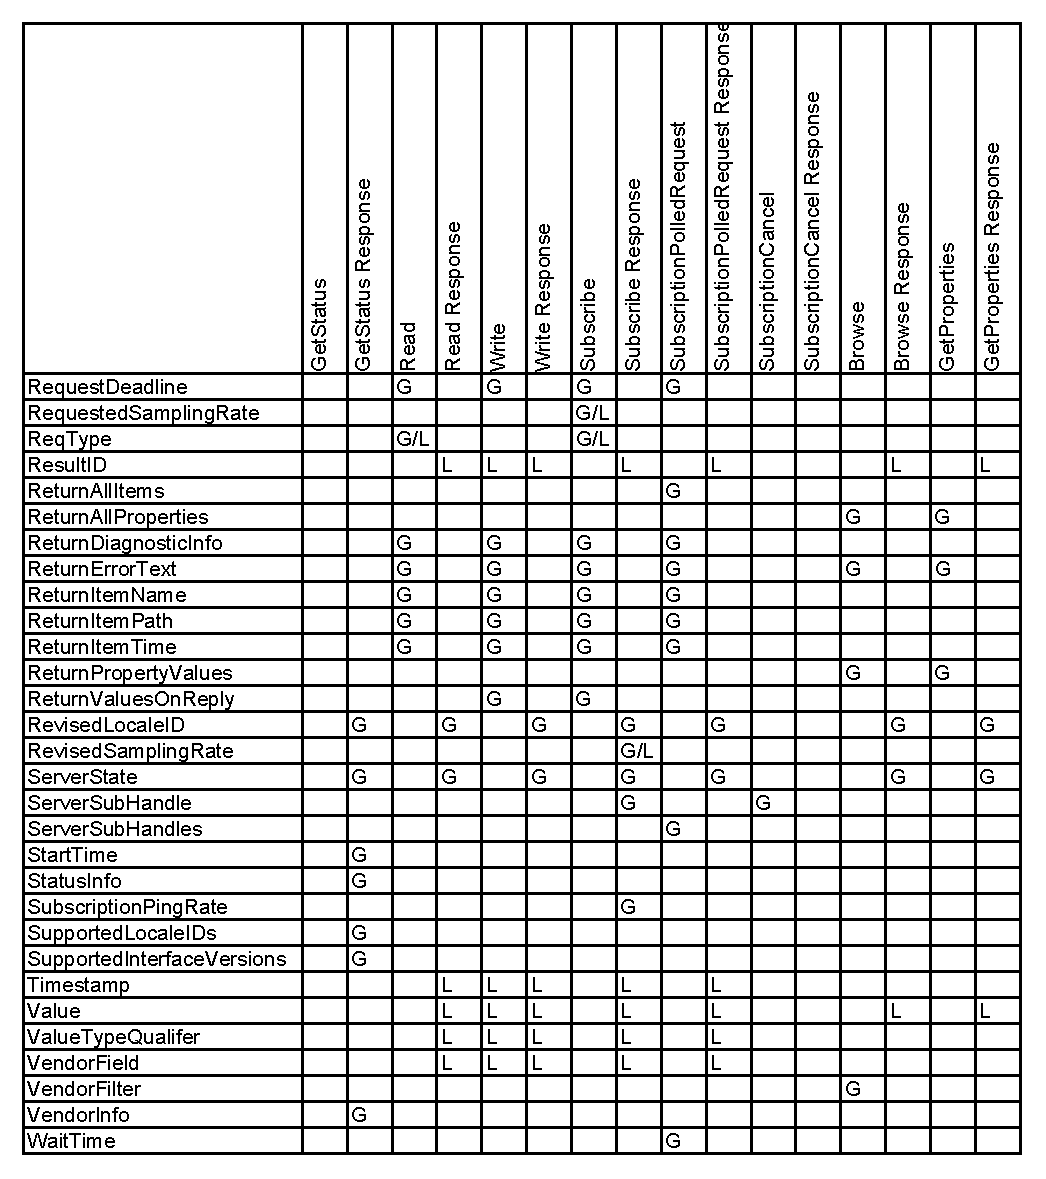
\includegraphics[scale=0.9]{graphics/operations2.eps}
\caption{OPC Options and Operations}
\label {operations2} 
\end{table}

Moreover an alphabetical reference of all available OPC options is
given in this appendix, which outlines the functionality of an OPC
option and moreover denotes, by which Python data type it is
represented in the PyOPC framework.


\begin{description}

\item[BrowseFilter] ({\sl string}) Limits the returned elements during
a browse operation. Allowed values are {\sl all, branch, item}.
\item[ClientItemHandle] ({\sl string}): An identifier of the item in a
request message. The ClientItemHandle is returned along with the
requested item.
\item[ClientRequestHandle] ({\sl string}): An identifier of the client
request.
\item[ContinuationPoint] ({\sl string}): A browse option for specifying
secondary browse requests.
\item[DataBufferOverflow] ({\sl bool}): Indicates if some item changes
were lost during subsequent subscription polls
\item[Deadband] ({\sl float}): The percentage of an item value change
which has to be exceeded so that the item ``has changed'', meaning
that the item will be sent during the next subscription poll.
\item[DiagnosticInfo] ({\sl string}): Additional server specific
information in case of an error.
\item[Description] ({\sl string}): A verbose description of an item
property
\item[ElementNameFilter] ({\sl string}): Limits the returned elements
during a browse operation
\item[EnableBuffering] ({\sl bool}): Denotes if changed values should
be buffered in case of a subscription
\item[ErrorText] ({\sl string}): Verbose error description in case of
an item error
\item[HasChildren] ({\sl bool}): Indicates if a browse element has
child elements
\item[HoldTime] ({\sl datetime}): Time to wait until the subscription poll
response is sent
\item[InvalidServerSubHandles] ({\sl list of strings}): A list of invalid
ServerSubHandles
\item[IsItem] ({\sl bool}): Indicates if a browse element is an item
\item[ItemName] ({\sl string}): The ItemName is part of the namespace
of an OPC item. Together with the ItemPath, it forms a unique
identification of an item.
\item[ItemPath] ({\sl string}): The ItemPath is part of the namespace
of an OPC item. Together with the ItemName, it forms a unique
identification of an item.
\item[LimitField] ({\sl string}): Transports the limit status of an
OPC item and may be one of the following string: {\sl none, low,
high, constant}.
\item[LocaleID] ({\sl string}): Requested locale for the return message.
\item[MaxAge] ({\sl long}): Denotes how old the item value may be in
milliseconds. MaxAge can be utilized for item caching in the server.

% A newpage is inserted as otherwise the inserted table leads to the 
% placement of the word ``request'' on the next page, which looks weird.
\newpage

\item[MaxElementsReturned] ({\sl long}): Maximum amount of returned
elements during a browse request.
\item[MoreElements] ({\sl bool}): Indicates that there are more
elements than the returned ones in a browse response message
\item[Name] ({\sl string/QName}): This option is used as an identifier
for a browse element (string type) or a property (QName type).
\item[ProductVersion] ({\sl string}): A version string of the OPC server
\item[PropertyNames] ({\sl list of QNames}): A list of item properties
that should be returned.
\item[QualityField] ({\sl string}): The quality of an OPC item value.
\cite{OPCXMLDA} specifies a predefined list of allowed qualities, such
as ``good'', ``uncertain'' or ``bad''.
\item[RcvTime] ({\sl datetime}): The time the server received the request.
\item[ReplyTime] ({\sl datetime}): The time the server returned the response.
\item[RequestDeadline] ({\sl datetime}): The time until the server
response has to be issued.
\item[RequestedSamplingRate] ({\sl long}): The time in milliseconds in
which the server checks for value changes in case of a subscription.
\item[ReqType] ({\sl QName}): With this options, the client may
specify the data type of an OPC item value. The available data types
are listed in \cite{OPCXMLDA}.
\item[ResultID] ({\sl QName}): In case of an item error, this option
specifies the error type.
\item[ReturnAllItems] ({\sl bool}): Indicates if the server should
return only the changed or all OPC items during a subscription poll
\item[ReturnAllProperties] ({\sl bool}): Indicates if all item
properties should be returned
\item[ReturnDiagnosticInfo] ({\sl bool}): Return additional server
specific information in case of an error
\item[ReturnErrorText] ({\sl bool}): If True, the OPC server returns a
verbose error description in case of an item error.
\item[ReturnItemName] ({\sl bool}): Indicates whether the ItemName
is returned by the server
\item[ReturnItemPath] ({\sl bool}): Indicates whether the ItemPath is
returned by the server
\item[ReturnItemTime] ({\sl bool}): Indicates whether the Timestamp of an
OPC item is returned by the server
\item[ReturnPropertyValues] ({\sl bool}): Indicates whether all item
property values should be included in a response message
\item[ReturnValuesOnReply] ({\sl bool}): Specifies if the item values
should be included in the response message
\item[RevisedLocaleID] ({\sl string}): In case the requested locale is not
implemented by the server, it is revised. The revised locale is sent back
to the client by the RevisedLocaleID option.
\item[RevisedSamplingRate] ({\sl long}): If the OPC server does not
the requested subscription sampling rate, it returns a revised rate in
this option.
\item[ServerState] ({\sl string}): The current status of the OPC
server, the values may be one of the following: {\sl running, failed,
noConfig, suspended, test, commFault}
\item[ServerSubHandle] ({\sl string}): An identifier of an OPC
subscription
\item[ServerSubHandles] ({\sl list of strings}): A list of
ServerSubHandles.
\item[StartTime] ({\sl datetime}): The time the OPC server was started
\item[StatusInfo] ({\sl string}): Provides additional server information.
\item[SubscriptionPingRate] ({\sl long}): Maximum time in milliseconds
between SubscriptionPolledRequest operations. If the ping rate is
exceeded, the subscription will be canceled.
\item[SupportedLocaleIDs] ({\sl string}): String that contains all
supported locales by the server
\item[SupportedInterfaceVersions] ({\sl string}): Supported versions
of the OPC XML-DA standard, currently only ``XML\_DA\_Version\_1\_0'' is
allowed
\item[Timestamp] ({\sl datetime}): The time when the OPC item value
was sampled
\item[Value] ({\sl anyType}): The value of an OPC item or OPC
property
\item[ValueTypeQualifier] ({\sl QName}): In case the value is
date/time based, it will identifiy the exact XML-Schema data type.
\item[VendorField] ({\sl long}): A numeric value that matches the OPC
Vendor Bit Field
\item[VendorFilter] ({\sl string}): Limits the returned elements
during a browse operation
\item[VendorInfo] ({\sl string}): Vendor specific server information
\item[WaitTime] ({\sl long}): Time in milliseconds which the server
should wait during a pending subscription poll for item value changes
\end{description}


\newpage

% Description: Bibliography
% Pagecount: -
%
%
\addcontentsline{toc}{section}{Bibliography}
\begin {thebibliography}{AAA11}

\bibitem[BIR01]{XML1} {\bf Mark Birbeck, Jason Diamond, Jon Ducket et al.}:\\
{\it Professional XML 2nd Edition}\\
Wrox Press Ltd. {\bf 2001}

\bibitem[FET06]{TWISTED} {\bf Abe Fettig}:\\
{\it Twisted Network Programming Essentials}
O'Reilly, CA-95472 {\bf 2006}

\bibitem[HIM06]{diplomarbeit} {\bf Hermann Himmelbauer}:\\
{\it SOAP Interface For An Internet/Fieldbus Gateway}
\\ Vienna University of Technology, Austria
{\bf 2006}

\bibitem[HUN03]{JUNIT} {\bf Andy Hunt / Dave Thomas}:\\
{\it Pragmatic Unit Testing in Java with JUnit}
The Pragmatic Programmers, LLC {\bf 2003}

\bibitem[LIV02]{SOAP2} {\bf Dan Livingston}:\\
{\it Advanced SOAP Web Development}\\
Prentice-Hall Inc., NJ-07458 {\bf 2002}

\bibitem[MAR03]{PYTHON} {\bf Alex Martelli}:\\
{\it Python in a Nutshell}\\
O'Reilly, CA-95472 {\bf 2003}

\bibitem[OPCDA]{OPCDA} {\bf OPC Foundation}:\\
{\it OPC Data Access Custom Interface Standard Version 3.00}\\
OPC Foundation, AZ-85260-1830, {\bf 2003}

\bibitem[OPCXMLDA]{OPCXMLDA} {\bf OPC Foundation}:\\
{\it OPC XML-DA Specification Version 1.01}\\ OPC Foundation,
AZ-85260-1830, {\bf 2004}

\bibitem[PIL05]{diveintopython} {\bf Mark Pilgrim}:\\
{\it Dive Into Python}\\
Apress CA-94710 {\bf 2005}

\bibitem[SEE02]{SOAP1} {\bf Scott Seely}:\\
{\it SOAP: Cross Platform Web Service Development using XML}\\
Prentice-Hall Inc., NJ-07458 {\bf 2002}

\bibitem[VLI02]{XSD1} {\bf Eric van der Vlist}:\\
{\it XML Schema}\\
O'Reilly, CA-95472 {\bf 2002}

\bibitem[WAL02]{SOAP4} {\bf Aaron E. Walsh}:\\
{\it UDDI, SOAP and WSDL - The Web Services Specification
Reference Book}\\
Prentice-Hall Inc., NJ-07458 {\bf 2002}

\end{thebibliography}

\newpage 
\end{appendix}
\end{document}
